\documentclass{beamer}

\usetheme{Hannover}
\usecolortheme{dove}

\usepackage{mhchem}
\usepackage{graphicx}
\usepackage{helvet}

\usepackage[german]{babel}
\usepackage[T1]{fontenc}
\usepackage[utf8]{inputenc}

\DeclareGraphicsRule{.tif}{png}{.png}{`convert #1 `dirname #1`/`basename #1 .tif`.png}

\title{Akkumulatoren}
\author{Leon Handreke}
\date{5. Februar 2010}

\begin{document}

\frame{\titlepage}

\frame{\tableofcontents}

\section{Geschichte}
\frame{
  \frametitle{Geschichte}
  \begin{itemize}
  \item 1789 - Luigi Galvani - Galvanisches Element
  \item 1802 - Wilhelm Ritter - Erste ``aufladbare'' Zelle
  \item 1850 - Josef Sinsteden - Bleiakkumulator
  \item 1866 - Werner von Siemens - Elektrischer Generator
  \end{itemize}

}
\section{Definition}
\frame
{
  \frametitle{Definition}
  \begin{quote}
    Ein Akkumulator ist ein Speicher für elektrische Energie, meist auf Basis eines elektrochemischen Systems.
  \end{quote}
  \small{Wikipedia}
}

\section{Bleiakku}
\frame{
  \frametitle{Bleiakku}
  \begin{itemize}
  \item Elektrolyt: Schwefelsäure (\ce{H2SO4})
  \item Spannung: 2V
  \item Pluspol: \ce{PbO2}
  \item Minuspol: \ce{Pb}
  \end{itemize}
}

\subsection{Ladung}
\frame{
  \frametitle{Bleiakku - Ladung}
  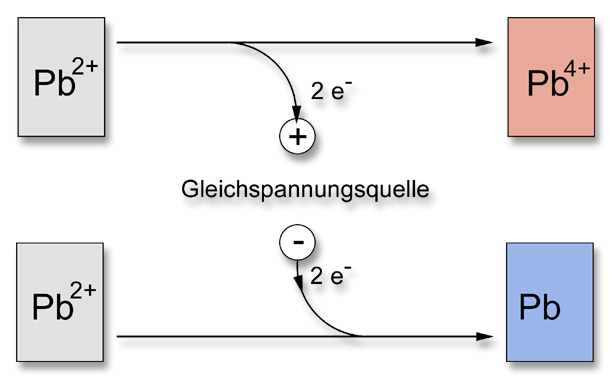
\includegraphics[width=\textwidth]{bleiakku-reaktion.png}
}

\subsection{Wirkung des Elektrolyts}
\frame{
  \frametitle{Wirkung des Elektrolyts}
  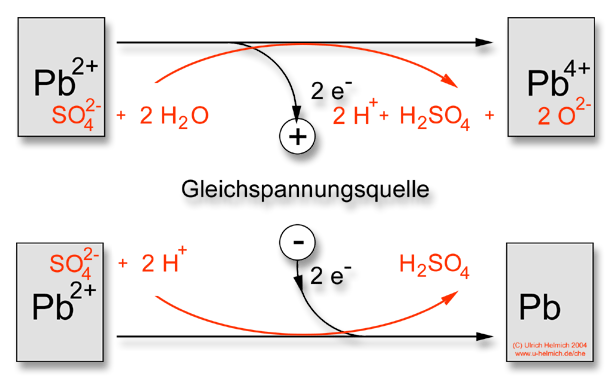
\includegraphics[width=\textwidth]{bleiakku-reaktion-elektrolyt.png}
}

\subsection{Entladung}
\frame{
  \frametitle{Bleiakku - Entladung}
  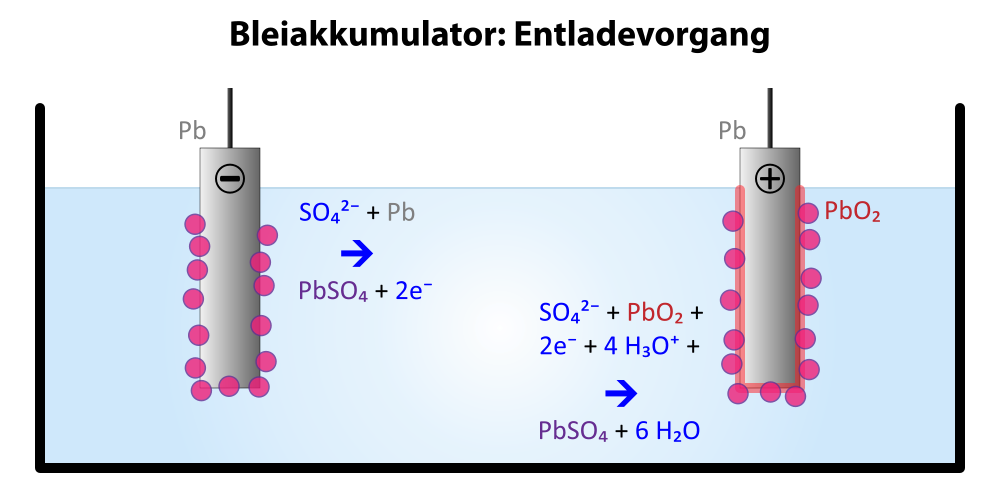
\includegraphics[width=\textwidth]{bleiakku-entladung.png}
}

\subsection{Spannung}
\frame{
  \frametitle{Spannung - Formel}
  $\Delta EMK = E ^{0} _{A} - E ^{0} _{D}$
}

\frame{
  \frametitle{Spannung - Rechnung}
  $\Delta EMK = E ^{0} _{\ce{Pb4+}} - E ^{0} _{\ce{Pb}}$
  
  $\Delta EMK = 1.8V - (-0.1262V) = 2V$
}

\subsection{Vor- und Nachteile}
\frame{
  \frametitle{Vorteile}
  \begin{itemize}
  \item Kurzzeitig hohe Stromstärken
  \item Kosteneffektiv
  \end{itemize}
}

\frame{
  \frametitle{Nachteile}
  \begin{itemize}
  \item Überladung: ``Gasen''
  \item Tiefentladung
  \item Kristallisierung von \ce{PbSO4}
  \end{itemize}
}


\section{Andere Akkumulatortypen}

\frame{
  \frametitle{Nickel-Cadmium}
  \begin{itemize}
  \item \ce{NiCd}
  \item 1.2V Spannung
  \item Geringe Kapazität
  \item EU-weites Verkaufsverbot seit 2009
  \end{itemize}
}

\frame{
  \frametitle{Nickel-Metallhydrid}
  \begin{itemize}
  \item \ce{NiMH}
  \item 1.2V Spannung
  \item ``Normale'' Haushaltsakkus
  \end{itemize}
}

\frame{
  \frametitle{Lithium-Ionen}
  \begin{itemize}
  \item \ce{LiIon}
  \item 3.62V Spannung
  \item Elektronische Geräte (Mobilfunkgeräte, Laptops...)
  \end{itemize}
}

\frame{
  \frametitle{Lithium-Polymer}
  \begin{itemize}
  \item \ce{LiPo}
  \item 3.7V Spannung
  \item Modellfluggeräte, Elektronische Geräte
  \item Sehr teuer
  \item Sehr leicht
  \end{itemize}
}

\frame{
  \frametitle{Vergleich verschiedener Akkumulatortypen}
  
\includegraphics[width=\textwidth]{vergleich-akkus.png}
}

\section{Quellen}
\frame{
  \frametitle{Quellen}
  \begin{itemize}
  \item http://www.u-helmich.de/che/09/04-ionen/ionen14.html
  \item http://de.wikipedia.org/wiki/Akkumulator
  \item http://de.wikipedia.org/wiki/Bleiakkumulator
  \item http://commons.wikimedia.org/ (Illustrationen)
  \end{itemize}
}
\end{document}
